\documentclass[12pt,a4paper,oneside]{extarticle}
\usepackage[left=20mm, right=20mm, top=1in, bottom=1.1in]{geometry}
\usepackage{amsmath, amsthm, amssymb}
\usepackage{amsfonts}
\usepackage{mathtools}
\usepackage{gensymb}
\usepackage[utf8]{inputenc}
\usepackage{fancyhdr}
\usepackage{float}
\usepackage{array}
\usepackage{lastpage}
\usepackage{tcolorbox}
\usepackage{tikz,tkz-tab}
\usepackage{hyperref}
\usepackage{venndiagram}
\usepackage{subcaption}
\usepackage{pythontex}
\usepackage{minted}
\usetikzlibrary{angles,patterns,calc}
\graphicspath{ {./images/} }

\newcommand{\tabularSize}{37em}

\newcommand{\ROMAN}[1]{%
  \textup{\uppercase\expandafter{\romannumeral#1}}%
}

\newcommand{\Vector}[1]{
\overrightarrow{#1}
}

\newcommand{\OR}{\vee}
\newcommand{\AND}{\wedge} 
\newcommand{\XOR}{\oplus}
\DeclareMathOperator{\lcm}{lcm}

\newcounter{problem}
\setcounter{problem}{1}

\newcommand{\solution}[2]{
  \begin{tcolorbox}
    \textbf{\theproblem. } #1
  \end{tcolorbox}
  \begin{center}\textbf{Solution.}\end{center}
  #2 \addtocounter{problem}{1}
}


\makeatletter
\DeclareFontFamily{U}{tipa}{}
\DeclareFontShape{U}{tipa}{m}{n}{<->tipa10}{}
\newcommand{\arc@char}{{\usefont{U}{tipa}{m}{n}\symbol{62}}}%

\newcommand{\arc}[1]{\mathpalette\arc@arc{#1}}

\newcommand{\arc@arc}[2]{%
  \sbox0{$\m@th#1#2$}%
  \vbox{
    \hbox{\resizebox{\wd0}{\height}{\arc@char}}
    \nointerlineskip
    \box0
  }%
}
\makeatother

\DeclarePairedDelimiter{\ceil}{\lceil}{\rceil}
\DeclarePairedDelimiter\floor{\lfloor}{\rfloor}

\title{\textbf{{\large CSE251: System Programming}\\Assignment 2 - bomblab}}
\author{Student name: Nguyen Minh Duc\\Student ID: 20202026}
\date{}


\begin{document}
\pagestyle{fancy}
\fancyhf{}
\renewcommand{\headrulewidth}{1pt}
\fancyhead[LE,LO]{\textbf{CSE251: System Programming}}
\fancyhead[RE,RO]{\textbf{Assignment 2 - bomblab}}
\fancyfoot[CE,CO]{\thepage}
\renewcommand{\footrulewidth}{1pt}
\makeatletter

%\renewcommand{\thesubsection}{\Alph{subsection}}

\maketitle

This paper contains solutions to the assignment 2 of System Programming course (Spring 2022) at UNIST, which is to defuse the binary bomb.

\tableofcontents

\newpage


\addcontentsline{toc}{section}{Introduction}
\section*{Introduction}
To begin with, let's first look at the source code \textbf{bomb.c}
\begin{minted}[frame=single,framesep=10pt]{c}
  input = read_line();             /* Get input                   */
  phase_1(input);                  /* Run the phase               */
  phase_defused();                 /* Drat!  They figured it out!
            * Let me know how they did it. */
  printf("Phase 1 defused. How about the next one?\n");

  /* The second phase is harder.  No one will ever figure out
    * how to defuse this... */
  input = read_line();
  phase_2(input);
  phase_defused();
  printf("That's number 2.  Keep going!\n");

  /* I guess this is too easy so far.  Some more complex code will
    * confuse people. */
  input = read_line();
  phase_3(input);
  phase_defused();
  printf("Halfway there!\n");

  /* Oh yeah?  Well, how good is your math?  Try on this saucy problem! */
  input = read_line();
  phase_4(input);
  phase_defused();
  printf("So you got that one.  Try this one.\n");
  
  /* Round and 'round in memory we go, where we stop, the bomb blows! */
  input = read_line();
  phase_5(input);
  phase_defused();
  printf("Good work!  On to the next...\n");

  /* This phase will never be used, since no one will get past the
    * earlier ones.  But just in case, make this one extra hard. */
  input = read_line();
  phase_6(input);
  phase_defused();
\end{minted}

We can see that the bomb has six phases, and each phase requires us to input a certain string to defuse. There are 6 functions correspoding to 6 phases: \begin{verbatim} phase_1, phase_2, phase_3, phase_4, phase_5, phase_6 \end{verbatim}

\newpage

\section{Phase 1}
This is the first phase of the binary bomb. The bomb will greet you with the following lines
\begin{minted}[frame=single,framesep=10pt]{bash}
  [edusc03-052@cheetah022 bomb52]$ ./bomb
  Welcome to my fiendish little bomb. You have 6 phases with
  which to blow yourself up. Have a nice day!
\end{minted}
Entering a random string ``123'' will result in an explosion.
\begin{minted}[frame=single,framesep=10pt]{bash}
  [edusc03-052@cheetah022 bomb52]$ ./bomb
  Welcome to my fiendish little bomb. You have 6 phases with
  which to blow yourself up. Have a nice day!
  123

  BOOM!!!
  The bomb has blown up.
  [edusc03-052@cheetah022 bomb52]$
\end{minted}
In order to obtain the correct string, we have to use the \textbf{gdb} tool. Now we know that the function that handle the first phase is \verb+phase_1+, we can set a breakpoint at that function. Starting the bomb with the command \verb+r+ and inputting the random string ```123''' again, we obtain
\begin{minted}[frame=single,framesep=10pt]{bash}
  [edusc03-052@cheetah022 bomb52]$ gdb bomb
  (gdb) b phase_1
  Breakpoint 1 at 0x400e63
  (gdb) r
  Starting program: /home/edusc03/edusc03-052/bomb52/bomb
  Welcome to my fiendish little bomb. You have 6 phases with
  which to blow yourself up. Have a nice day!
  123

  Breakpoint 1, 0x0000000000400e63 in phase_1 ()
  (gdb)
\end{minted}
Disassembling the function, we have
\begin{minted}[frame=single,framesep=10pt]{bash}
  (gdb) disas
  Dump of assembler code for function phase_1:
  => 0x0000000000400e63 <+0>:     sub    $0x8,%rsp
     0x0000000000400e67 <+4>:     mov    $0x402330,%esi
     0x0000000000400e6c <+9>:     callq  0x401354 <strings_not_equal>
     0x0000000000400e71 <+14>:    test   %eax,%eax
     0x0000000000400e73 <+16>:    jne    0x400e7a <phase_1+23>
     0x0000000000400e75 <+18>:    add    $0x8,%rsp
     0x0000000000400e79 <+22>:    retq
     0x0000000000400e7a <+23>:    callq  0x401451 <explode_bomb>
     0x0000000000400e7f <+28>:    jmp    0x400e75 <phase_1+18>
  End of assembler dump.
\end{minted}
As the name suggests, the intruction \verb+callq  0x401354 <strings_not_equal>+ might compare two strings to see whether they are not equal. The previous instruction \verb+mov $0x402330,%esi+ also suggests one of the arguments will be in the address \verb+$0x402330+. By examining the address with the command \textbf{x/s}, we obtain the following string
\begin{minted}[frame=single,framesep=10pt]{bash}
  (gdb) x/s 0x402330
  0x402330:       "Verbosity leads to unclear, inarticulate things."
\end{minted}
which has a high chance to be the desired string. The following lines conducts an if-else statement, if the function returns true, the bomb will detonate, otherwise, the phase will be defused. Let's investigate the \verb+strings_not_equal+ function
\begin{minted}[frame=single,framesep=10pt]{bash}
  (gdb) disas strings_not_equal
  Dump of assembler code for function strings_not_equal:
    0x0000000000401354 <+0>:     push   %r12
    0x0000000000401356 <+2>:     push   %rbp
    0x0000000000401357 <+3>:     push   %rbx
    0x0000000000401358 <+4>:     mov    %rdi,%rbx
    0x000000000040135b <+7>:     mov    %rsi,%rbp
    0x000000000040135e <+10>:    callq  0x401337 <string_length>
    0x0000000000401363 <+15>:    mov    %eax,%r12d
    0x0000000000401366 <+18>:    mov    %rbp,%rdi
    0x0000000000401369 <+21>:    callq  0x401337 <string_length>
    0x000000000040136e <+26>:    mov    $0x1,%edx
    0x0000000000401373 <+31>:    cmp    %eax,%r12d
    0x0000000000401376 <+34>:    je     0x40137f <strings_not_equal+43>
  ---Type <return> to continue, or q <return> to quit---q
\end{minted}
It is clear that the function is comparing the two strings reside in \verb+%rdi+ and \verb+%rsi+ registers. By a direct examination, we obtain the two strings
\begin{minted}[frame=single,framesep=10pt]{bash}
  (gdb) x/s $rsi
  0x402330:       "Verbosity leads to unclear, inarticulate things."
  (gdb) x/s $rdi
  0x6037a0 <input_strings>:       "123"
\end{minted}
of which one of them is our inputted string. We can conclude that for any string we entered, the bomb compares it with the string ``Verbosity leads to unclear, inarticulate things.''\\
Reset the bomb and enter the newly found string, we have defused the first phase
\begin{minted}[frame=single,framesep=10pt]{bash}
  [edusc03-052@cheetah022 bomb52]$ ./bomb
  Welcome to my fiendish little bomb. You have 6 phases with
  which to blow yourself up. Have a nice day!
  Verbosity leads to unclear, inarticulate things.
  Phase 1 defused. How about the next one?
\end{minted}

\newpage
\section{Phase 2}
This is the second phase of the binary bomb. The bomb will greet you with the following lines
\begin{minted}[frame=single,framesep=10pt]{bash}
  [edusc03-052@cheetah022 bomb52]$ ./bomb
  Welcome to my fiendish little bomb. You have 6 phases with
  which to blow yourself up. Have a nice day!
  Verbosity leads to unclear, inarticulate things.
  Phase 1 defused. How about the next one?
\end{minted}
let's first open the \textbf{gdb} tool up, examine and put a breakpoint at the function \verb+phase_2+
\begin{minted}[frame=single,framesep=10pt]{bash}
  (gdb) r
  Starting program: /home/edusc03/edusc03-052/bomb52/bomb
  Welcome to my fiendish little bomb. You have 6 phases with
  which to blow yourself up. Have a nice day!
  Verbosity leads to unclear, inarticulate things.
  Phase 1 defused. How about the next one?
  123

  Breakpoint 1, 0x0000000000400e81 in phase_2 ()
  (gdb) disas
  Dump of assembler code for function phase_2:
  => 0x0000000000400e81 <+0>:     push   %rbx
     0x0000000000400e82 <+1>:     sub    $0x20,%rsp
     0x0000000000400e86 <+5>:     mov    %rsp,%rsi
     0x0000000000400e89 <+8>:     callq  0x401473 <read_six_numbers>
     0x0000000000400e8e <+13>:    cmpl   $0x0,(%rsp)
     0x0000000000400e92 <+17>:    js     0x400e9b <phase_2+26>
     0x0000000000400e94 <+19>:    mov    $0x1,%ebx
     0x0000000000400e99 <+24>:    jmp    0x400eac <phase_2+43>
     0x0000000000400e9b <+26>:    callq  0x401451 <explode_bomb>
     0x0000000000400ea0 <+31>:    jmp    0x400e94 <phase_2+19>
     0x0000000000400ea2 <+33>:    add    $0x1,%rbx
     0x0000000000400ea6 <+37>:    cmp    $0x6,%rbx
     0x0000000000400eaa <+41>:    je     0x400ebe <phase_2+61>
     0x0000000000400eac <+43>:    mov    %ebx,%eax
     0x0000000000400eae <+45>:    add    -0x4(%rsp,%rbx,4),%eax
     0x0000000000400eb2 <+49>:    cmp    %eax,(%rsp,%rbx,4)
     0x0000000000400eb5 <+52>:    je     0x400ea2 <phase_2+33>
     0x0000000000400eb7 <+54>:    callq  0x401451 <explode_bomb>
     0x0000000000400ebc <+59>:    jmp    0x400ea2 <phase_2+33>
     0x0000000000400ebe <+61>:    add    $0x20,%rsp
     0x0000000000400ec2 <+65>:    pop    %rbx
     0x0000000000400ec3 <+66>:    retq
  End of assembler dump.
\end{minted}
Again, the function tries to call another function, this time is \verb+read_six_numbers+. Let's examine it
\begin{minted}[frame=single,framesep=10pt]{bash}
  (gdb) disas read_six_numbers
  Dump of assembler code for function read_six_numbers:
     0x0000000000401473 <+0>:     sub    $0x8,%rsp
     0x0000000000401477 <+4>:     mov    %rsi,%rdx
     0x000000000040147a <+7>:     lea    0x4(%rsi),%rcx
     0x000000000040147e <+11>:    lea    0x14(%rsi),%rax
     0x0000000000401482 <+15>:    push   %rax
     0x0000000000401483 <+16>:    lea    0x10(%rsi),%rax
     0x0000000000401487 <+20>:    push   %rax
     0x0000000000401488 <+21>:    lea    0xc(%rsi),%r9
     0x000000000040148c <+25>:    lea    0x8(%rsi),%r8
     0x0000000000401490 <+29>:    mov    $0x402523,%esi
     0x0000000000401495 <+34>:    mov    $0x0,%eax
     0x000000000040149a <+39>:    callq  0x400bc0 <__isoc99_sscanf@plt>
     0x000000000040149f <+44>:    add    $0x10,%rsp
     0x00000000004014a3 <+48>:    cmp    $0x5,%eax
     0x00000000004014a6 <+51>:    jle    0x4014ad <read_six_numbers+58>
     0x00000000004014a8 <+53>:    add    $0x8,%rsp
     0x00000000004014ac <+57>:    retq
     0x00000000004014ad <+58>:    callq  0x401451 <explode_bomb>
  End of assembler dump.
\end{minted}
We can see that the function tries to invoke \verb+__isoc99_sscanf+ function. The first few lines of the function load data into registers and push some of them on the stack. The name of those registers suggests that they contain arguments to be passed into \verb+sscanf+. As we know, it takes in at least two arguments, a string $s$ and an C-formatted pattern $p$, and returns the number of matches in $s$ according to the pattern $p$. Note that the values in the address \verb+0x402523+ is moved into the \verb+%esi+ register, which is usually an argument. Inspect that memory, we obtain
\begin{minted}[frame=single,framesep=10pt]{bash}
  (gdb) x/s 0x402523
  0x402523:       "%d %d %d %d %d %d"
\end{minted}
which suggests that the desired string should contain six 32-bit integers separated by spaces. The last few lines construct an if-else statement, which is roughly translated into C as
\begin{minted}[frame=single,framesep=10pt]{c}
  if(eax > 5){ // eax = return value of __isoc99_sscanf
    return;
  }
  explode_bomb();
\end{minted}
We will pass this stage if $\text{eax} > 5$, i.e, the number of integers in our string is at least 6. If we continue to run our debugger, the bomb will explode since our first guess only contains one integer $123$.\\
Reset the bomb and type in ``1 2 3 4 5 6'', we now have passed the \verb+read_six_numbers+ function. The remainning lines of codes seem comlicated, let's explore them part by part. Firstly, let's inspect what's residing in the \verb+%rsp+ register
\begin{minted}[frame=single,framesep=10pt]{bash}
  (gdb) x $rsp
  0x7fffffffe210: 0x00000001
\end{minted}
If we reset the bomb again and enter ``0 1 2 3 4 5'', we obtain another value of \verb+rsp+ in this stage
\begin{minted}[frame=single,framesep=10pt]{bash}
  (gdb) x $rsp
  0x7fffffffe210: 0x00000000
\end{minted}
which is the same as the first integer we have just inputted. To confirm our hypothesis that \verb+rsp+ contains the six inputted integers, we type in the command \verb+x/6d+ in gdb
\begin{minted}[frame=single,framesep=10pt]{bash}
  (gdb) x/6d $rsp
  0x7fffffffe210: 1       2       3       4
  0x7fffffffe220: 5       6
\end{minted}
Now we know that \verb+rsp+ holds our input, let's carry on with the following lines
{\renewcommand\fcolorbox[4][]{\textcolor{cyan}{\strut#4}}
\begin{minted}[frame=single,framesep=10pt]{gas}
  0x0000000000400e8e <+13>:    cmpl   $0x0,(%rsp)
  0x0000000000400e92 <+17>:    js     0x400e9b <phase_2+26>  
\end{minted}
}\noindent
This checks if the first number is less than $0$. If it is, then the bomb will detonate, otherwise, it will continue with the following instructions
{\renewcommand\fcolorbox[4][]{\textcolor{cyan}{\strut#4}}
\begin{minted}[frame=single,framesep=10pt]{gas}
  0x0000000000400e94 <+19>:    mov    $0x1,%ebx
  0x0000000000400e99 <+24>:    jmp    0x400eac <phase_2+43>
  0x0000000000400e9b <+26>:    callq  0x401451 <explode_bomb>
  0x0000000000400ea0 <+31>:    jmp    0x400e94 <phase_2+19>
  0x0000000000400ea2 <+33>:    add    $0x1,%rbx
  0x0000000000400ea6 <+37>:    cmp    $0x6,%rbx
  0x0000000000400eaa <+41>:    je     0x400ebe <phase_2+61>
  0x0000000000400eac <+43>:    mov    %ebx,%eax
  0x0000000000400eae <+45>:    add    -0x4(%rsp,%rbx,4),%eax
  0x0000000000400eb2 <+49>:    cmp    %eax,(%rsp,%rbx,4)
  0x0000000000400eb5 <+52>:    je     0x400ea2 <phase_2+33>
  0x0000000000400eb7 <+54>:    callq  0x401451 <explode_bomb>
  0x0000000000400ebc <+59>:    jmp    0x400ea2 <phase_2+33>
\end{minted}
}
This part of the code is the most complicated. It has a lot of backward jumps, so it might be a loop. Further investigation confirms our hypothesis. First, \verb+ebx+ is initialized to $1$ and the value is moved to \verb+eax+. Then, the bomb executes \verb+add -0x4(%rsp,%rbx,4),%eax+, which can be translated into C code as: $\verb+eax+ \mathrel{+}= \verb+rsp+[\verb+rbx+ - 1]$, assuming that everything is of type \verb+int+. Next, the bomb will compare \verb+eax+ with $\verb+rsp+[\verb+rbx+]$, if they are equal, we continue with the line 33, otherwise, the bomb will explode. Lastly, the bomb will increment \verb+rbx+ and check if it is equal to $6$. If it is, the loop will terminate and phase 2 is defused, otherwise, the loop will continue. In summary, the assembly code can be roughly translated into the following C code
\begin{minted}[frame=single,framesep=10pt]{c}
  // suppose that a[6] is the array that contains the input
  int i = 1;
  do{
    if(i + a[i - 1] != a[i]) explode_bomb();
    i += 1;
  } while(i != 6);
\end{minted}
This gives us a recurrence formula for the desired series of integers
$$ a_n = \begin{cases}
  c & \text{if }n = 0,\\
  a_{n - 1} + n & \text{otherwise},
\end{cases} $$
for any arbitary integer $c \geq 0$. Solving this recurrence formula, we obtain the result
$$ a_n = c + \dfrac{n(n + 1)}{2}. $$
This suggests that there's more than one solution to this phase. For simplicity, let's choose $c = 0$, reset the bomb and input the string ``0 1 3 6 10 15'', which will defuse the second phase of the bomb.
{\renewcommand\fcolorbox[4][]{\textcolor{black}{\strut#4}}
\begin{minted}[frame=single,framesep=10pt]{bash}
  [edusc03-052@cheetah022 bomb52]$ ./bomb
  Welcome to my fiendish little bomb. You have 6 phases with
  which to blow yourself up. Have a nice day!
  Verbosity leads to unclear, inarticulate things.
  Phase 1 defused. How about the next one?
  0 1 3 6 10 15
  That's number 2.  Keep going!
\end{minted}
}

\newpage
\section{Phase 3}
This is the third phase of the binary bomb. The bomb will greet you with the following lines
{\renewcommand\fcolorbox[4][]{\textcolor{black}{\strut#4}}
\begin{minted}[frame=single,framesep=10pt]{bash}
  [edusc03-052@cheetah022 bomb52]$ ./bomb  input.txt
  Welcome to my fiendish little bomb. You have 6 phases with
  which to blow yourself up. Have a nice day!
  Phase 1 defused. How about the next one?
  That's number 2.  Keep going!
  1 2 3 4 5 6
\end{minted}
}\noindent
Let's entered a dummy string into the bomb, i.e. ``1 2 3 4 5 6''.\\
As usual, let's investigate the phase by \textbf{gdb}. Since the assembly code is too long, I will break it down into different sections.
{\renewcommand\fcolorbox[4][]{\textcolor{cyan}{\strut#4}}
\begin{minted}[frame=single,framesep=10pt]{gas}
  0x0000000000400ec4 <+0>:     sub    $0x18,%rsp
  0x0000000000400ec8 <+4>:     lea    0x8(%rsp),%r8
  0x0000000000400ecd <+9>:     lea    0x7(%rsp),%rcx
  0x0000000000400ed2 <+14>:    lea    0xc(%rsp),%rdx
  0x0000000000400ed7 <+19>:    mov    $0x40238e,%esi
  0x0000000000400edc <+24>:    mov    $0x0,%eax
  0x0000000000400ee1 <+29>:    callq  0x400bc0 <__isoc99_sscanf@plt>
  0x0000000000400ee6 <+34>:    cmp    $0x2,%eax
  0x0000000000400ee9 <+37>:    jle    0x400f01 <phase_3+61>
\end{minted}
}\noindent
As we can see, this function also invoke \verb+sscanf+, let's investigate what is the pattern \verb+sscanf+ takes as argument
{\renewcommand\fcolorbox[4][]{\textcolor{cyan}{\strut#4}}
\begin{minted}[frame=single,framesep=10pt]{bash}
  (gdb) x/s 0x40238e
  0x40238e:       "%d %c %d"
\end{minted}
}\noindent
This implies that our input should have \verb+int+, \verb+char+, and \verb+int+ respectively. Since our dummy input satisfies the constraint, we pass this stage.\\
The next two lines also form an if-else statement. If \verb+0xc(%rsp)+$ > 7$, the bomb will explode, otherwise, it will move the data into \verb+%eax+ and continue into the next stage.
{\renewcommand\fcolorbox[4][]{\textcolor{cyan}{\strut#4}}
\begin{minted}[frame=single,framesep=10pt]{gas}
  0x0000000000400eeb <+39>:    cmpl   $0x7,0xc(%rsp)
  0x0000000000400ef0 <+44>:    ja     0x400ff9 <phase_3+309>
  0x0000000000400ef6 <+50>:    mov    0xc(%rsp),%eax
  0x0000000000400efa <+54>:    jmpq   *0x4023a0(,%rax,8)
\end{minted}
}\noindent
Let's explore what's inside \verb+0xc(%rsp)+ and \verb+0x4023a0+
\begin{minted}[frame=single,framesep=10pt]{bash}
  (gdb) x $rsp + 0xc
  0x7fffffffe22c: 0x00000001 # our first integer
  (gdb) x 0x4023a0
  0x4023a0:       0x0000000000400f08
\end{minted}
The last instruction jumps to the $*(\verb+0x4023a0+ + 8 \times$ \verb+%rax+$)$ line, where \verb+%rax+ is our first integer. This kind of behavior suggests a switch statement in C. Since \verb+%rax+ must be less than $7$, there are only eight cases needed to be handled, i.e. from $0$ to $7$.
\begin{minted}[frame=single,framesep=10pt]{c}
  switch(/*our first integer*/){
    case 0: // do something
    case 1: // do something
    case 2: // do something
    case 3: // do something
    case 4: // do something
    case 5: // do something
    case 6: // do something
    case 7: // do something
    default: explode_bomb();
  }
\end{minted}
In our dummy input, our first number is $1$, so we jump to the line \verb|0x0000000000400f2a <+102>|
{\renewcommand\fcolorbox[4][]{\textcolor{cyan}{\strut#4}}
\begin{minted}[frame=single,framesep=10pt]{gas}
  0x0000000000400f2a <+102>:   mov    $0x72,%eax
  0x0000000000400f2f <+107>:   cmpl   $0x10f,0x8(%rsp)
  0x0000000000400f37 <+115>:   je     0x401003 <phase_3+319>
  0x0000000000400f3d <+121>:   callq  0x401451 <explode_bomb>
\end{minted}
}\noindent
Let's first see what's inside \verb+0x8(%rsp)+
\begin{minted}[frame=single,framesep=10pt]{bash}
  (gdb) print *(int*)(0x8 + $rsp)
  $17 = 3
\end{minted}
which is our third integer. Now, let's translate the above assembly code into C code
\begin{minted}[frame=single,framesep=10pt]{c}
  case 1:
    eax = 0x72;
    if(0x10f != *(rsp + 0x8)) explode_bomb();
    break;
\end{minted}
This means that our third number must be equal to \verb+0x10f+, i.e. $271$, which is not the case here. Let's reset the bomb and modify the input string
{\renewcommand\fcolorbox[4][]{\textcolor{black}{\strut#4}}
\begin{minted}[frame=single,framesep=10pt]{bash}
  Welcome to my fiendish little bomb. You have 6 phases with
  which to blow yourself up. Have a nice day!
  Verbosity leads to unclear, inarticulate things.
  Phase 1 defused. How about the next one?
  0 1 3 6 10 15
  That's number 2.  Keep going!
  1 a 271
\end{minted}
}\noindent
We have now passed the switch statement, and left with just a few instructions
{\renewcommand\fcolorbox[4][]{\textcolor{cyan}{\strut#4}}
\begin{minted}[frame=single,framesep=10pt]{gas}
  0x0000000000401003 <+319>:   cmp    %al,0x7(%rsp)
  0x0000000000401007 <+323>:   je     0x40100e <phase_3+330>
  0x0000000000401009 <+325>:   callq  0x401451 <explode_bomb>
  0x000000000040100e <+330>:   add    $0x18,%rsp
  0x0000000000401012 <+334>:   retq
\end{minted}
}\noindent
It's comparing two values at \verb+%al+ and \verb+0x7(%rsp)+. Let's see what's in \verb+0x7(%rsp)+
\begin{minted}[frame=single,framesep=10pt]{bash}
  (gdb) x (int*)(0x7 + $rsp)
  0x7fffffffe227: 97 'a'
\end{minted}
which is our second input character. As for the register \verb+%al+
\begin{minted}[frame=single,framesep=10pt]{bash}
  (gdb) print (char)$al
  $21 = 114 'r'
\end{minted}
So now, we know that the second character must be `\verb+r+'. Resetting the bomb and entering the string ``1 r 271'', we have now defused the third phase.
{\renewcommand\fcolorbox[4][]{\textcolor{black}{\strut#4}}
\begin{minted}[frame=single,framesep=10pt]{bash}
  [edusc03-052@cheetah022 bomb52]$ ./bomb input.txt
  Welcome to my fiendish little bomb. You have 6 phases with
  which to blow yourself up. Have a nice day!
  Phase 1 defused. How about the next one?
  That's number 2.  Keep going!
  1 r 271
  Halfway there!
\end{minted}
}\noindent

\newpage
\section{Phase 4}
This is the forth phase of the binary bomb. The bomb will greet you with the following lines
{\renewcommand\fcolorbox[4][]{\textcolor{black}{\strut#4}}
\begin{minted}[frame=single,framesep=10pt]{bash}
  [edusc03-052@cheetah022 bomb52]$ ./bomb input.txt
  Welcome to my fiendish little bomb. You have 6 phases with
  which to blow yourself up. Have a nice day!
  Phase 1 defused. How about the next one?
  That's number 2.  Keep going!
  Halfway there!
\end{minted}
}\noindent
Let's entered a dummy string into the bomb, i.e. ``1 2 3''. Now, we obtain the following assembly code
{\renewcommand\fcolorbox[4][]{\textcolor{cyan}{\strut#4}}
\begin{minted}[frame=single,framesep=10pt]{gas}
  0x0000000000401047 <+0>:     sub    $0x18,%rsp
  0x000000000040104b <+4>:     lea    0x8(%rsp),%rcx
  0x0000000000401050 <+9>:     lea    0xc(%rsp),%rdx
  0x0000000000401055 <+14>:    mov    $0x40252f,%esi
  0x000000000040105a <+19>:    mov    $0x0,%eax
  0x000000000040105f <+24>:    callq  0x400bc0 <__isoc99_sscanf@plt>
  0x0000000000401064 <+29>:    cmp    $0x2,%eax
  0x0000000000401067 <+32>:    jne    0x401070 <phase_4+41>
  0x0000000000401069 <+34>:    cmpl   $0xe,0xc(%rsp)
  0x000000000040106e <+39>:    jbe    0x401075 <phase_4+46>
  0x0000000000401070 <+41>:    callq  0x401451 <explode_bomb>
  0x0000000000401075 <+46>:    mov    $0xe,%edx
  0x000000000040107a <+51>:    mov    $0x0,%esi
  0x000000000040107f <+56>:    mov    0xc(%rsp),%edi
  0x0000000000401083 <+60>:    callq  0x401013 <func4>
  0x0000000000401088 <+65>:    cmp    $0x12,%eax
  0x000000000040108b <+68>:    jne    0x401094 <phase_4+77>
  0x000000000040108d <+70>:    cmpl   $0x12,0x8(%rsp)
  0x0000000000401092 <+75>:    je     0x401099 <phase_4+82>
  0x0000000000401094 <+77>:    callq  0x401451 <explode_bomb>
  0x0000000000401099 <+82>:    add    $0x18,%rsp
  0x000000000040109d <+86>:    retq
\end{minted}
}\noindent
Again, the function tries to invoke \verb+sscanf+, let's see what's the pattern
{\renewcommand\fcolorbox[4][]{\textcolor{cyan}{\strut#4}}
\begin{minted}[frame=single,framesep=10pt]{bash}
  (gdb) x/s 0x40252f
  0x40252f:       "%d %d"
\end{minted}
}\noindent
which implies our input should contain two 32-bit integer. The two lines
{\renewcommand\fcolorbox[4][]{\textcolor{cyan}{\strut#4}}
\begin{minted}[frame=single,framesep=10pt]{gas}
  0x0000000000401064 <+29>:    cmp    $0x2,%eax
  0x0000000000401067 <+32>:    jne    0x401070 <phase_4+41>
\end{minted}
}\noindent
say that if we do not meet the criteria, the bomb will explode. Luckily, our dummy input statisfies the first constraint. Next, there're these two lines
{\renewcommand\fcolorbox[4][]{\textcolor{cyan}{\strut#4}}
\begin{minted}[frame=single,framesep=10pt]{gas}
  0x0000000000401069 <+34>:    cmpl   $0xe,0xc(%rsp)
  0x000000000040106e <+39>:    jbe    0x401075 <phase_4+46>
  0x0000000000401070 <+41>:    callq  0x401451 <explode_bomb>
\end{minted}
}\noindent
comparing \verb+0xc(%rsp)+ with \verb+0xe+, i.e. $14$. Let's investigate \verb+0xc(%rsp)+
{\renewcommand\fcolorbox[4][]{\textcolor{black}{\strut#4}}
\begin{minted}[frame=single,framesep=10pt]{bash}
  (gdb) x/d (0xc + $rsp)
  0x7fffffffe22c: 1
\end{minted}
}\noindent
which is our first integer. So if our first integer is bigger than $14$, the bomb will also detonate. Next, let's examine the following lines
{\renewcommand\fcolorbox[4][]{\textcolor{cyan}{\strut#4}}
\begin{minted}[frame=single,framesep=10pt]{gas}
  0x0000000000401075 <+46>:    mov    $0xe,%edx
  0x000000000040107a <+51>:    mov    $0x0,%esi
  0x000000000040107f <+56>:    mov    0xc(%rsp),%edi
  0x0000000000401083 <+60>:    callq  0x401013 <func4>
\end{minted}
}\noindent
It calls another function \verb+func4+ that takes in $3$ arguments, \verb+0xe+, \verb+0x0+, and our first number. Dive in \verb+func4+
{\renewcommand\fcolorbox[4][]{\textcolor{cyan}{\strut#4}}
\begin{minted}[frame=single,framesep=10pt]{gas}
  0x0000000000401013 <+0>:     push   %rbx
  0x0000000000401014 <+1>:     mov    %edx,%eax
  0x0000000000401016 <+3>:     sub    %esi,%eax
  0x0000000000401018 <+5>:     mov    %eax,%ebx
  0x000000000040101a <+7>:     shr    $0x1f,%ebx
  0x000000000040101d <+10>:    add    %eax,%ebx
  0x000000000040101f <+12>:    sar    %ebx
  0x0000000000401021 <+14>:    add    %esi,%ebx
  0x0000000000401023 <+16>:    cmp    %edi,%ebx
  0x0000000000401025 <+18>:    jg     0x40102f <func4+28>
  0x0000000000401027 <+20>:    cmp    %edi,%ebx
  0x0000000000401029 <+22>:    jl     0x40103b <func4+40>
  0x000000000040102b <+24>:    mov    %ebx,%eax
  0x000000000040102d <+26>:    pop    %rbx
  0x000000000040102e <+27>:    retq
  0x000000000040102f <+28>:    lea    -0x1(%rbx),%edx
  0x0000000000401032 <+31>:    callq  0x401013 <func4>
  0x0000000000401037 <+36>:    add    %eax,%ebx
  0x0000000000401039 <+38>:    jmp    0x40102b <func4+24>
  0x000000000040103b <+40>:    lea    0x1(%rbx),%esi
  0x000000000040103e <+43>:    callq  0x401013 <func4>
  0x0000000000401043 <+48>:    add    %eax,%ebx
  0x0000000000401045 <+50>:    jmp    0x40102b <func4+24>
\end{minted}
}\noindent
We can see that it calls itself at the line $31$ and $43$, so it is a recursive function. Note that it takes $3$ arguments, let's call them $x, y, z$, which are \verb+%edx+, \verb+%esi+, and \verb+%edi+ respectively. Firstly, let's try to understand these first lines of codes
{\renewcommand\fcolorbox[4][]{\textcolor{cyan}{\strut#4}}
\begin{minted}[frame=single,framesep=10pt]{gas}
  0x0000000000401014 <+1>:     mov    %edx,%eax
  0x0000000000401016 <+3>:     sub    %esi,%eax
  0x0000000000401018 <+5>:     mov    %eax,%ebx
  0x000000000040101a <+7>:     shr    $0x1f,%ebx
  0x000000000040101d <+10>:    add    %eax,%ebx
  0x000000000040101f <+12>:    sar    %ebx
  0x0000000000401021 <+14>:    add    %esi,%ebx
\end{minted}
}\noindent
which can be translated line by line as
{\renewcommand\fcolorbox[4][]{\textcolor{black}{\strut#4}}
\begin{minted}[frame=single,framesep=10pt]{c}
  eax = edx;
  eax -= esi;
  ebx = eax;
  ebx = (unsigned)ebx >> 0x1f;
  ebx += eax;
  ebx >>= 1;
  ebx += esi;
\end{minted}
}\noindent
let's instroduce new variables and subtitute $x, y, z$ in the correct registers
{\renewcommand\fcolorbox[4][]{\textcolor{black}{\strut#4}}
\begin{minted}[frame=single,framesep=10pt]{c}
  int a = x - y;
  int b = a;
  b = (unsigned)b >> 0x1f;
  b += a;
  b >>= 1;
  b += y;
\end{minted}
}\noindent
The next instructions construct an if-else statement
{\renewcommand\fcolorbox[4][]{\textcolor{cyan}{\strut#4}}
\begin{minted}[frame=single,framesep=10pt]{gas}
  0x0000000000401023 <+16>:    cmp    %edi,%ebx
  0x0000000000401025 <+18>:    jg     0x40102f <func4+28>
  0x0000000000401027 <+20>:    cmp    %edi,%ebx
  0x0000000000401029 <+22>:    jl     0x40103b <func4+40>
  0x000000000040102b <+24>:    mov    %ebx,%eax
  0x000000000040102d <+26>:    pop    %rbx
  0x000000000040102e <+27>:    retq
\end{minted}
}\noindent
Let's translate into C:
{\renewcommand\fcolorbox[4][]{\textcolor{black}{\strut#4}}
\begin{minted}[frame=single,framesep=10pt]{c}
  if(b > z){
    // func4+28
  } else if(b < z){
    // func4+40
  }
  a = b;
  return a;
\end{minted}
}\noindent
Let's explore the line 28 of the function
{\renewcommand\fcolorbox[4][]{\textcolor{cyan}{\strut#4}}
\begin{minted}[frame=single,framesep=10pt]{gas}
  0x000000000040102f <+28>:    lea    -0x1(%rbx),%edx
  0x0000000000401032 <+31>:    callq  0x401013 <func4>
  0x0000000000401037 <+36>:    add    %eax,%ebx
  0x0000000000401039 <+38>:    jmp    0x40102b <func4+24>
\end{minted}
}\noindent
Translating into C, we obtain
{\renewcommand\fcolorbox[4][]{\textcolor{black}{\strut#4}}
\begin{minted}[frame=single,framesep=10pt]{c}
  x = b - 1;
  a = func4(x, y, z);
  b += a;
\end{minted}
}\noindent
As for the line 40:
{\renewcommand\fcolorbox[4][]{\textcolor{cyan}{\strut#4}}
\begin{minted}[frame=single,framesep=10pt]{gas}
  0x000000000040103b <+40>:    lea    0x1(%rbx),%esi
  0x000000000040103e <+43>:    callq  0x401013 <func4>
  0x0000000000401043 <+48>:    add    %eax,%ebx
  0x0000000000401045 <+50>:    jmp    0x40102b <func4+24>
\end{minted}
}\noindent
Translating into C, we obtain
{\renewcommand\fcolorbox[4][]{\textcolor{black}{\strut#4}}
\begin{minted}[frame=single,framesep=10pt]{c}
  y = b + 1;
  a = func4(x, y, z);
  b += a;
\end{minted}
}\noindent
Now, we have completely reverse engineered \verb+func4+. The C code is as follow
{\renewcommand\fcolorbox[4][]{\textcolor{black}{\strut#4}}
\begin{minted}[frame=single,framesep=10pt]{c}
  int func4(int x, int y, int z){
    int a = x - y;
    int b = a;
    b = (unsigned)b >> 31;
    b += a;
    b >>= 1;
    b += y;
    if(b - z > 0){
        x = b - 1;
        a = func4(x, y, z);
        b += a;
    } else if(b - z < 0){
        y = b + 1;
        a = func4(x, y, z);
        b += a;
    }
    a = b;
    return a;
  }
\end{minted}
}\noindent
Now, we have known what \verb+func4+ is doing, let's continue with the assembly code of \verb+phase_4+
{\renewcommand\fcolorbox[4][]{\textcolor{cyan}{\strut#4}}
\begin{minted}[frame=single,framesep=10pt]{gas}
  0x0000000000401088 <+65>:    cmp    $0x12,%eax
  0x000000000040108b <+68>:    jne    0x401094 <phase_4+77>
  0x000000000040108d <+70>:    cmpl   $0x12,0x8(%rsp)
  0x0000000000401092 <+75>:    je     0x401099 <phase_4+82>
  0x0000000000401094 <+77>:    callq  0x401451 <explode_bomb>
  0x0000000000401099 <+82>:    add    $0x18,%rsp
  0x000000000040109d <+86>:    retq
\end{minted}
}\noindent
where \verb+%eax+ is the returned value of \verb+func4+. If it is not \verb+0x12+, i.e. $18$, then the bomb will explode, otherwise, it continue to compare \verb+0x8(%rsp)+ with $18$. Let's see what's inside
\begin{minted}[frame=single,framesep=10pt]{bash}
  (gdb) x/d (0x8+$rsp)
  0x7fffffffe228: 2
\end{minted}
which is our second integer. So if it is not the same as $18$, the bomb will detonate, otherwise, we successfully defuse the bomb. The only problem left is that what should the first number, let's call it $z$, be in order for the output of \verb+func4+ to be $18$. Fortunately, we know the range of the input, which is $z \leq 14$, and we also know the C code of \verb+func4+. The task is now trivial as we only need to bruteforce through $15$ different values of $z$, i.e. $\{0, 1, 2, \dots, 14\}$ with a simple C code
{\renewcommand\fcolorbox[4][]{\textcolor{black}{\strut#4}}
\begin{minted}[frame=single,framesep=10pt]{c}
#include <stdio.h>
int func4(int x, int y, int z){
    int a = x - y;
    int b = a;
    b = (unsigned)b >> 31;
    b += a; b >>= 1; b += y;
    if(b > z){
        a = func4(b - 1, y, z);
        b += a;
    } else if(b < z){
        a = func4(x, b + 1, z);
        b += a;
    }
    a = b;
    return a;
}
int main() {
    for(int i = 0; i <= 14; i++)
        printf("i = %d -> %d\n", i, func4(14, 0, i));
    return 0;
}
\end{minted}
}\noindent
The output is
\begin{minted}[frame=single,framesep=10pt]{bash}
  i = 0 -> 11
  i = 1 -> 11
  i = 2 -> 13
  i = 3 -> 10
  i = 4 -> 19
  i = 5 -> 15
  i = 6 -> 21
  i = 7 -> 7
  i = 8 -> 35
  i = 9 -> 27
  i = 10 -> 37
  i = 11 -> 18
  i = 12 -> 43
  i = 13 -> 31
  i = 14 -> 45
\end{minted}
From this, we know that our first number should be $11$. Resetting the bomb and enter ``\verb+11 18+'', this phase will be defused successfully.
{\renewcommand\fcolorbox[4][]{\textcolor{black}{\strut#4}}
\begin{minted}[frame=single,framesep=10pt]{bash}
  [edusc03-052@cheetah022 bomb52]$ ./bomb input.txt
  Welcome to my fiendish little bomb. You have 6 phases with
  which to blow yourself up. Have a nice day!
  Phase 1 defused. How about the next one?
  That's number 2.  Keep going!
  Halfway there!
  11 18
  So you got that one.  Try this one.
\end{minted}
}


\newpage
\section{Phase 5}
This is the fifth phase of the binary bomb. The bomb will greet you with the following lines
{\renewcommand\fcolorbox[4][]{\textcolor{black}{\strut#4}}
\begin{minted}[frame=single,framesep=10pt]{bash}
  [edusc03-052@cheetah022 bomb52]$ ./bomb input.txt
  Welcome to my fiendish little bomb. You have 6 phases with
  which to blow yourself up. Have a nice day!
  Phase 1 defused. How about the next one?
  That's number 2.  Keep going!
  Halfway there!
  So you got that one.  Try this one.
\end{minted}
}\noindent
As usual, let's enter a dummy input ``1 2'' and inspect the phase's assembly code
{\renewcommand\fcolorbox[4][]{\textcolor{cyan}{\strut#4}}
\begin{minted}[frame=single,framesep=10pt]{gas}
  0x000000000040109e <+0>:     sub    $0x18,%rsp
  0x00000000004010a2 <+4>:     lea    0x8(%rsp),%rcx
  0x00000000004010a7 <+9>:     lea    0xc(%rsp),%rdx
  0x00000000004010ac <+14>:    mov    $0x40252f,%esi
  0x00000000004010b1 <+19>:    mov    $0x0,%eax
  0x00000000004010b6 <+24>:    callq  0x400bc0 <__isoc99_sscanf@plt>
  0x00000000004010bb <+29>:    cmp    $0x1,%eax
  0x00000000004010be <+32>:    jle    0x40110a <phase_5+108>
  0x00000000004010c0 <+34>:    mov    0xc(%rsp),%eax
  0x00000000004010c4 <+38>:    and    $0xf,%eax
  0x00000000004010c7 <+41>:    mov    %eax,0xc(%rsp)
  0x00000000004010cb <+45>:    cmp    $0xf,%eax
  0x00000000004010ce <+48>:    je     0x401100 <phase_5+98>
  0x00000000004010d0 <+50>:    mov    $0x0,%ecx
  0x00000000004010d5 <+55>:    mov    $0x0,%edx
  0x00000000004010da <+60>:    add    $0x1,%edx
  0x00000000004010dd <+63>:    cltq
  0x00000000004010df <+65>:    mov    0x4023e0(,%rax,4),%eax
  0x00000000004010e6 <+72>:    add    %eax,%ecx
  0x00000000004010e8 <+74>:    cmp    $0xf,%eax
  0x00000000004010eb <+77>:    jne    0x4010da <phase_5+60>
  0x00000000004010ed <+79>:    movl   $0xf,0xc(%rsp)
  0x00000000004010f5 <+87>:    cmp    $0xf,%edx
  0x00000000004010f8 <+90>:    jne    0x401100 <phase_5+98>
  0x00000000004010fa <+92>:    cmp    %ecx,0x8(%rsp)
  0x00000000004010fe <+96>:    je     0x401105 <phase_5+103>
  0x0000000000401100 <+98>:    callq  0x401451 <explode_bomb>
  0x0000000000401105 <+103>:   add    $0x18,%rsp
  0x0000000000401109 <+107>:   retq
  0x000000000040110a <+108>:   callq  0x401451 <explode_bomb>
  0x000000000040110f <+113>:   jmp    0x4010c0 <phase_5+34>
\end{minted}
}\noindent
This function also calls \verb+sscanf+, let's see what's the pattern
{\renewcommand\fcolorbox[4][]{\textcolor{cyan}{\strut#4}}
\begin{minted}[frame=single,framesep=10pt]{bash}
  (gdb) x/s 0x40252f
  0x40252f:       "%d %d"
\end{minted}
}\noindent
So our dummy input statisfies the first constraint. Next, let's inspect the following lines
{\renewcommand\fcolorbox[4][]{\textcolor{cyan}{\strut#4}}
\begin{minted}[frame=single,framesep=10pt]{gas}
  0x00000000004010c0 <+34>:    mov    0xc(%rsp),%eax
  0x00000000004010c4 <+38>:    and    $0xf,%eax
  0x00000000004010c7 <+41>:    mov    %eax,0xc(%rsp)
  0x00000000004010cb <+45>:    cmp    $0xf,%eax
  0x00000000004010ce <+48>:    je     0x401100 <phase_5+98>
\end{minted}
}\noindent
It moves something into the \verb+%eax+ register, and conduct an \verb+AND+ operation with \verb+0xf+, i.e. 15, or equivalently in base 2: \verb+1111+. This effectively is a modulo operation mod $2^4 = 16$. Then, it move the data back into \verb+0xc(%rsp)+. The last two lines form an if statement, if the register is the same as $15$, the bomb will explode, otherwise, we are good to go to the next state of the bomb. Let's first check what's inside \verb+0xc(%rsp)+
{\renewcommand\fcolorbox[4][]{\textcolor{cyan}{\strut#4}}
\begin{minted}[frame=single,framesep=10pt]{bash}
  (gdb) x/d (0xc + $rsp)
  0x7fffffffe22c: 1
\end{minted}
}\noindent
which is our first number. Thus, our dummy input statisfies this second constraint. Let's continue with the next lines of assembly codes
{\renewcommand\fcolorbox[4][]{\textcolor{cyan}{\strut#4}}
\begin{minted}[frame=single,framesep=10pt]{gas}
  0x00000000004010d0 <+50>:    mov    $0x0,%ecx
  0x00000000004010d5 <+55>:    mov    $0x0,%edx
  0x00000000004010da <+60>:    add    $0x1,%edx
  0x00000000004010dd <+63>:    cltq
  0x00000000004010df <+65>:    mov    0x4023e0(,%rax,4),%eax
  0x00000000004010e6 <+72>:    add    %eax,%ecx
  0x00000000004010e8 <+74>:    cmp    $0xf,%eax
  0x00000000004010eb <+77>:    jne    0x4010da <phase_5+60>
  0x00000000004010ed <+79>:    movl   $0xf,0xc(%rsp)
  0x00000000004010f5 <+87>:    cmp    $0xf,%edx
  0x00000000004010f8 <+90>:    jne    0x401100 <phase_5+98>
\end{minted}
}\noindent
This portion of the phase has a backward jump, so it might be a loop. Initially, there's two register \verb+%ecx+ and \verb+%edx+ both are assigned to $0$. Then, the loop starts with the incrementation of \verb+%edx+. The bomb move a value into the \verb+%eax+ register, let's investigate it.
{\renewcommand\fcolorbox[4][]{\textcolor{cyan}{\strut#4}}
\begin{minted}[frame=single,framesep=10pt]{bash}
  (gdb) x 0x4023e0 + 4*$rax
  0x4023e4 <array.3237+4>:        2
\end{minted}
}\noindent
What's an interesting name, \verb+array.3237+. We know that \verb+%rax+ contains our first number, and \verb+(,%rax,4)+ is an offset from the ``array'', so it might be the index of the ``array''. Let's confirm our guess by examining the address \verb+0x4023e0+
{\renewcommand\fcolorbox[4][]{\textcolor{cyan}{\strut#4}}
\begin{minted}[frame=single,framesep=10pt]{bash}
  (gdb) x/100d 0x4023e0
  0x4023e0 <array.3237>:    10 0 0 0 2  0 0 0
  0x4023e8 <array.3237+8>:  14 0 0 0 7  0 0 0
  0x4023f0 <array.3237+16>: 8  0 0 0 12 0 0 0
  0x4023f8 <array.3237+24>: 15 0 0 0 11 0 0 0
  0x402400 <array.3237+32>: 0  0 0 0 4  0 0 0
  0x402408 <array.3237+40>: 1  0 0 0 13 0 0 0
  0x402410 <array.3237+48>: 3  0 0 0 9  0 0 0
  0x402418 <array.3237+56>: 6  0 0 0 5  0 0 0
  0x402420: 83  111 32  121 111 117 32  116
  0x402428: 104 105 110 107 32  121 111 117
  0x402430: 32  99  97  110 32  115 116 111
  0x402438: 112 32  116 104 101 32  98  111
  0x402440: 109 98  32  119
\end{minted}
}\noindent
From this data, we can conclude that there's an array of size $16$ and it's elements are
{\renewcommand\fcolorbox[4][]{\textcolor{black}{\strut#4}}
\begin{minted}[frame=single,framesep=10pt]{c}
  int array[] = {10, 2, 14, 7, 8, 12, 15, 11, 0, 4, 1, 13, 3, 9, 6, 5};
\end{minted}
}\noindent
The next line is pretty simple, it adds \verb+%eax+ into \verb+%ecx+, compares whether \verb+%eax+ is $15$, if it is, terminate the loop, otherwise, continue the loop. Out side the loop, it assigns \verb+0xc(%rsp)+ to $15$ and compares \verb+%edx+ with $15$. If they are not equal, the bomb will detonate, otherwise nothing happens. All of this reasoning can be translated into C code as
{\renewcommand\fcolorbox[4][]{\textcolor{black}{\strut#4}}
\begin{minted}[frame=single,framesep=10pt]{c}
  // Let x be our first number
  int cnt, sum;
  int array[] = {10, 2, 14, 7, 8, 12, 15, 11, 0, 4, 1, 13, 3, 9, 6, 5};
  cnt = 0; sum = 0;
  do{
    int p = array[x];
    sum += p;
    x = p;
  } while(x != 15);
  x = 15;
  if(cnt != 15) bomb_explode();
\end{minted}
}\noindent
This behavior is a traversal through out the array using their values as the next index to visit. The below is the graph of this structure
\begin{center}
  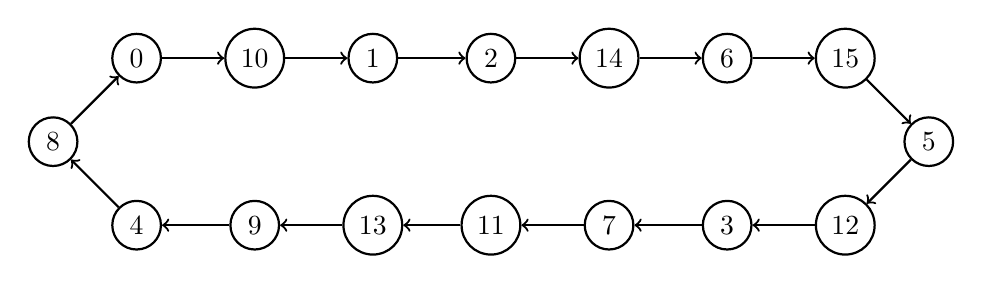
\begin{tikzpicture}[node distance={15mm}, thick, main/.style = {draw, circle}] 
    \node[main] (0) {$0$};
    \node[main] (10) [right of = 0] {$10$};
    \node[main] (1) [right of = 10] {$1$};
    \node[main] (2) [right of = 1] {$2$};
    \node[main] (14) [right of = 2] {$14$};
    \node[main] (6) [right of = 14] {$6$};
    \node[main] (15) [right of = 6] {$15$};
    \node[main] (5) [below right of = 15] {$5$};
    \node[main] (12) [below left of = 5] {$12$};
    \node[main] (3) [left of = 12] {$3$};
    \node[main] (7) [left of = 3] {$7$};
    \node[main] (11) [left of = 7] {$11$};
    \node[main] (13) [left of = 11] {$13$};
    \node[main] (9) [left of = 13] {$9$};
    \node[main] (4) [left of = 9] {$4$};
    \node[main] (8) [above left of = 4] {$8$};
    
    \draw[->] (0) -- (10);
    \draw[->] (10) -- (1);
    \draw[->] (1) -- (2);
    \draw[->] (2) -- (14);
    \draw[->] (14) -- (6);
    \draw[->] (6) -- (15);
    \draw[->] (15) -- (5);
    \draw[->] (5) -- (12);
    \draw[->] (12) -- (3);
    \draw[->] (3) -- (7);
    \draw[->] (7) -- (11);
    \draw[->] (11) -- (13);
    \draw[->] (13) -- (9);
    \draw[->] (9) -- (4);
    \draw[->] (4) -- (8);
    \draw[->] (8) -- (0);
  \end{tikzpicture} 
\end{center}
The code tells us that the traversal terminates when it reaches the node $15$. If all of the nodes are not visited, the bomb will explode, so we need to find a starting point such that it will visit every nodes. Fortunately, this is trivial, as we just need to look at the graph, which is the node $5$. So our first number should be $5$. Reset the bomb and type in ``5 6'' will pass this loop. Let's focus on the last lines
{\renewcommand\fcolorbox[4][]{\textcolor{cyan}{\strut#4}}
\begin{minted}[frame=single,framesep=10pt]{gas}
  0x00000000004010fa <+92>:    cmp    %ecx,0x8(%rsp)
  0x00000000004010fe <+96>:    je     0x401105 <phase_5+103>
  0x0000000000401100 <+98>:    callq  0x401451 <explode_bomb>
  0x0000000000401105 <+103>:   add    $0x18,%rsp
  0x0000000000401109 <+107>:   retq
\end{minted}
}\noindent
From the code above, we know that \verb+%ecx+ is the sum of the nodes that we passed through, let's inspect \verb+0x8(%rsp)+, and \verb+%ecx+
{\renewcommand\fcolorbox[4][]{\textcolor{cyan}{\strut#4}}
\begin{minted}[frame=single,framesep=10pt]{bash}
  (gdb) x 0x8+$rsp
  0x7fffffffe228: 6 # our second input
  (gdb) print $ecx
  $1 = 115
\end{minted}
}\noindent
Therefore, we obtain the correct input for this phase is ``5 115''. Resetting the bomb and type in ``5 115'', we have successfully defused the bomb.
{\renewcommand\fcolorbox[4][]{\textcolor{cyan}{\strut#4}}
\begin{minted}[frame=single,framesep=10pt]{bash}
  [edusc03-052@cheetah022 bomb52]$ ./bomb input.txt
  Welcome to my fiendish little bomb. You have 6 phases with
  which to blow yourself up. Have a nice day!
  Phase 1 defused. How about the next one?
  That's number 2.  Keep going!
  Halfway there!
  So you got that one.  Try this one.
  5 115
  Good work!  On to the next...
\end{minted}
}\noindent
\newpage
\section{Phase 6}
This is the last phase of the binary bomb. The bomb will greet you with the following lines
{\renewcommand\fcolorbox[4][]{\textcolor{black}{\strut#4}}
\begin{minted}[frame=single,framesep=10pt]{bash}
  [edusc03-052@cheetah022 bomb52]$ ./bomb input.txt
  Welcome to my fiendish little bomb. You have 6 phases with
  which to blow yourself up. Have a nice day!
  Phase 1 defused. How about the next one?
  That's number 2.  Keep going!
  Halfway there!
  So you got that one.  Try this one.
  Good work!  On to the next...
\end{minted}
}\noindent
Again, let's enter a dummy input ``1 2'' into the bomb, and investigate the assembly code. Since the assembly code is too long, I will break it down into different sections.
{\renewcommand\fcolorbox[4][]{\textcolor{cyan}{\strut#4}}
\begin{minted}[frame=single,framesep=10pt]{gas}
  0x0000000000401111 <+0>:     push   %r14
  0x0000000000401113 <+2>:     push   %r13
  0x0000000000401115 <+4>:     push   %r12
  0x0000000000401117 <+6>:     push   %rbp
  0x0000000000401118 <+7>:     push   %rbx
  0x0000000000401119 <+8>:     sub    $0x50,%rsp
  0x000000000040111d <+12>:    lea    0x30(%rsp),%rsi
  0x0000000000401122 <+17>:    callq  0x401473 <read_six_numbers>
  0x0000000000401127 <+22>:    lea    0x30(%rsp),%r12
  0x000000000040112c <+27>:    mov    %r12,%r13
  0x000000000040112f <+30>:    mov    $0x0,%r14d
  0x0000000000401135 <+36>:    jmp    0x40115d <phase_6+76>
  0x0000000000401137 <+38>:    callq  0x401451 <explode_bomb>
\end{minted}
}\noindent
We meet the function \verb+read_six_numbers+ again, which will detonate the bomb if we entered less than 6 integers. Let's reset the bomb and type ``1 2 3 4 5 6'' into the bomb, which will get us pass this first stage of the phase. Next, the bomb load \verb+0x30(%rsp)+ into the register \verb+r12+, let's see what's inside
{\renewcommand\fcolorbox[4][]{\textcolor{black}{\strut#4}}
\begin{minted}[frame=single,framesep=10pt]{bash}
  (gdb) x (0x30+$rsp)
  0x7fffffffe1f0: 0x00000001
\end{minted}
}\noindent
which is our first integer. Then, the bomb will jump to line 76. Let's go to it
{\renewcommand\fcolorbox[4][]{\textcolor{cyan}{\strut#4}}
\begin{minted}[frame=single,framesep=10pt]{gas}
  0x000000000040115d <+76>:    mov    %r13,%rbp
  0x0000000000401160 <+79>:    mov    0x0(%r13),%eax
  0x0000000000401164 <+83>:    sub    $0x1,%eax
  0x0000000000401167 <+86>:    cmp    $0x5,%eax
  0x000000000040116a <+89>:    ja     0x401137 <phase_6+38>
  0x000000000040116c <+91>:    add    $0x1,%r14d
  0x0000000000401170 <+95>:    cmp    $0x6,%r14d
  0x0000000000401174 <+99>:    je     0x40117b <phase_6+106>
  0x0000000000401176 <+101>:   mov    %r14d,%ebx
  0x0000000000401179 <+104>:   jmp    0x401146 <phase_6+53>
\end{minted}
}\noindent
Note that there's two backward jumps, so it might be a loop. After the first two lines, \verb+eax+ is holding our first integer, then, it got decremented and compared with $5$. if it is more than $5$, we jump to the line 38, which is \verb|explode_bomb|, otherwise, we continue with the next lines. Initially, \verb|r14d| is $0$, now it is incremented and compared with $6$, if they are equal, the loop will terminate, otherwise, the bomb assigns the value to \verb|ebx| and continues the loop.
{\renewcommand\fcolorbox[4][]{\textcolor{cyan}{\strut#4}}
\begin{minted}[frame=single,framesep=10pt]{gas}
  0x0000000000401146 <+53>:    movslq %ebx,%rax
  0x0000000000401149 <+56>:    mov    0x30(%rsp,%rax,4),%eax
  0x000000000040114d <+60>:    cmp    %eax,0x0(%rbp)
  0x0000000000401150 <+63>:    jne    0x40113e <phase_6+45>
  0x0000000000401152 <+65>:    callq  0x401451 <explode_bomb>
  0x0000000000401157 <+70>:    jmp    0x40113e <phase_6+45>
  0x0000000000401159 <+72>:    add    $0x4,%r13
\end{minted}
}\noindent
Let's inspect what's residing in \verb|0x30(%rsp,%rax,4)| and \verb|%rbp|
{\renewcommand\fcolorbox[4][]{\textcolor{black}{\strut#4}}
\begin{minted}[frame=single,framesep=10pt]{bash}
  (gdb) x/d $rbp
  0x7fffffffe1f0: 1
  (gdb) x/d $rsp+$rax*4+0x30
  0x7fffffffe1f4: 2
\end{minted}
}\noindent
which is our first and the next number. If they are equal, the bomb will explode, otherwise we go to the line 45
{\renewcommand\fcolorbox[4][]{\textcolor{cyan}{\strut#4}}
\begin{minted}[frame=single,framesep=10pt]{gas}
  0x000000000040113e <+45>:    add    $0x1,%ebx
  0x0000000000401141 <+48>:    cmp    $0x5,%ebx
  0x0000000000401144 <+51>:    jg     0x401159 <phase_6+72>
\end{minted}
}\noindent
Here, \verb|ebx| is incremented and compared with $5$, if it's greater than 5, we go to the line 72, otherwise, continue with the line 53 like above, which continues the loop.\\
This behavior suggest a nested loop, which can be roughly translated into C as
{\renewcommand\fcolorbox[4][]{\textcolor{black}{\strut#4}}
\begin{minted}[frame=single,framesep=10pt]{c}
  // Let's suppose that a[6] = {our 6 numbers}
  int i = 0, j = 0;
  while(i < 6){
    if(a[i] > 6) explode_bomb();
    j = i;
    while(j < 6){
      if(a[i] == a[j]) explode_bomb();
      j++;
    }
    i++;
  }
\end{minted}
}\noindent
In conclusion, this part is for checking whether all the numbers in the input is less than or equal to $6$ and all of them are pairwise distinct, i.e. a permutation from $1$ to $6$. Since our dummy input satisfies this constraint, we can pass this stage.
{\renewcommand\fcolorbox[4][]{\textcolor{cyan}{\strut#4}}
\begin{minted}[frame=single,framesep=10pt]{gas}
  0x000000000040117b <+106>:   lea    0x18(%r12),%rcx
  0x0000000000401180 <+111>:   mov    $0x7,%edx
  0x0000000000401185 <+116>:   mov    %edx,%eax
  0x0000000000401187 <+118>:   sub    (%r12),%eax
  0x000000000040118b <+122>:   mov    %eax,(%r12)
  0x000000000040118f <+126>:   add    $0x4,%r12
  0x0000000000401193 <+130>:   cmp    %r12,%rcx
  0x0000000000401196 <+133>:   jne    0x401185 <phase_6+116>
  0x0000000000401198 <+135>:   mov    $0x0,%esi
  0x000000000040119d <+140>:   jmp    0x4011b8 <phase_6+167>
\end{minted}
}\noindent
This also has a backward jump, so it has a high chance to be
Note that \verb|%r12| is the address of our first number, so \verb|%rcx| is the address that is after our last number.
{\renewcommand\fcolorbox[4][]{\textcolor{black}{\strut#4}}
\begin{minted}[frame=single,framesep=10pt]{bash}
  (gdb) x/8d $r12
  0x7fffffffe1f0: 1       2       3       4
  0x7fffffffe200: 5       6       6306096 0
\end{minted}
}\noindent
Next, \verb|edx| will be equal to \verb|0x7|, and then be assigned to \verb|eax|. Then, \verb|eax| will be subtracted by \verb|r12|, which is our first number, and it will be moved back to \verb|r12|. Finally. \verb|r12| is incremented by $4$, to our second integer. In conlusion, our 6 numbers are modified by the following function
$$ f(x) = 7 - x, $$
where $x$ is our input numbers. After this, our input will become $\{6, 5, 4, 3, 2, 1\}$. Now, let's continue with our bomb.
{\renewcommand\fcolorbox[4][]{\textcolor{cyan}{\strut#4}}
\begin{minted}[frame=single,framesep=10pt]{gas}
  0x00000000004011b8 <+167>:   mov    0x30(%rsp,%rsi,4),%ecx
  0x00000000004011bc <+171>:   mov    $0x1,%eax
  0x00000000004011c1 <+176>:   mov    $0x6032f0,%edx
  0x00000000004011c6 <+181>:   cmp    $0x1,%ecx
  0x00000000004011c9 <+184>:   jg     0x40119f <phase_6+142>
  0x00000000004011cb <+186>:   jmp    0x4011aa <phase_6+153>
\end{minted}
}\noindent
Let's see what's inside the address \verb|0x30(%rsp,%rsi,4)|
{\renewcommand\fcolorbox[4][]{\textcolor{black}{\strut#4}}
\begin{minted}[frame=single,framesep=10pt]{bash}
(gdb) x/8d (0x30+$rsp + $rsi * 4)
0x7fffffffe1f0: 6       5       4       3
0x7fffffffe200: 2       1       6306096 0
\end{minted}
}\noindent
which is our input. This lines of codes can be translated to C as follow
{\renewcommand\fcolorbox[4][]{\textcolor{black}{\strut#4}}
\begin{minted}[frame=single,framesep=10pt]{c}
  // Let a[6] = {our input numbers}
  ecx = a[0];
  eax = 1;
  edx = *0x6032f0;
  if(ecx > 1){
    // Line 142
  } else{
    // Line 153
  }
\end{minted}
}\noindent
Let's inspect \verb|0x6032f0|
{\renewcommand\fcolorbox[4][]{\textcolor{black}{\strut#4}}
\begin{minted}[frame=single,framesep=10pt]{bash}
  (gdb) x 0x6032f0
  0x6032f0 <node1>:       385
\end{minted}
}\noindent
What an interesting name, \verb|node1|. This suggest that it could be some data structures that related to nodes such as linked list, binary tree. Let's examine the address around it
{\renewcommand\fcolorbox[4][]{\textcolor{black}{\strut#4}}
\begin{minted}[frame=single,framesep=10pt]{bash}
  (gdb) x/30x 0x6032f0
  0x6032f0 <node1>: 0x00000181 0x00000001 0x00603300 0x00000000
  0x603300 <node2>: 0x0000010c 0x00000002 0x00603310 0x00000000
  0x603310 <node3>: 0x00000356 0x00000003 0x00603320 0x00000000
  0x603320 <node4>: 0x00000125 0x00000004 0x00603330 0x00000000
  0x603330 <node5>: 0x000003bd 0x00000005 0x00603340 0x00000000
  0x603340 <node6>: 0x000003bb 0x00000006 0x00000000 0x00000000
  0x603350 <bomb_id>: 0x00000034 0x00000000 0x00000000 0x00000000
  0x603360 <host_table>: 0x00402589 0x00000000
\end{minted}
}\noindent
From this, we know that there are $6$ nodes, and each of them as $4$ attributes. However, the last attribute is all $0$, so it does not serve any practical purpose. Hence, there's only $3$ active attributes. The second column is ranging from $1$ to $6$, so it might be the node's id. The third one looks like address values. Further investigation shows that it actually the address of the next node. The below is the diagram of the nodes
\begin{center}
  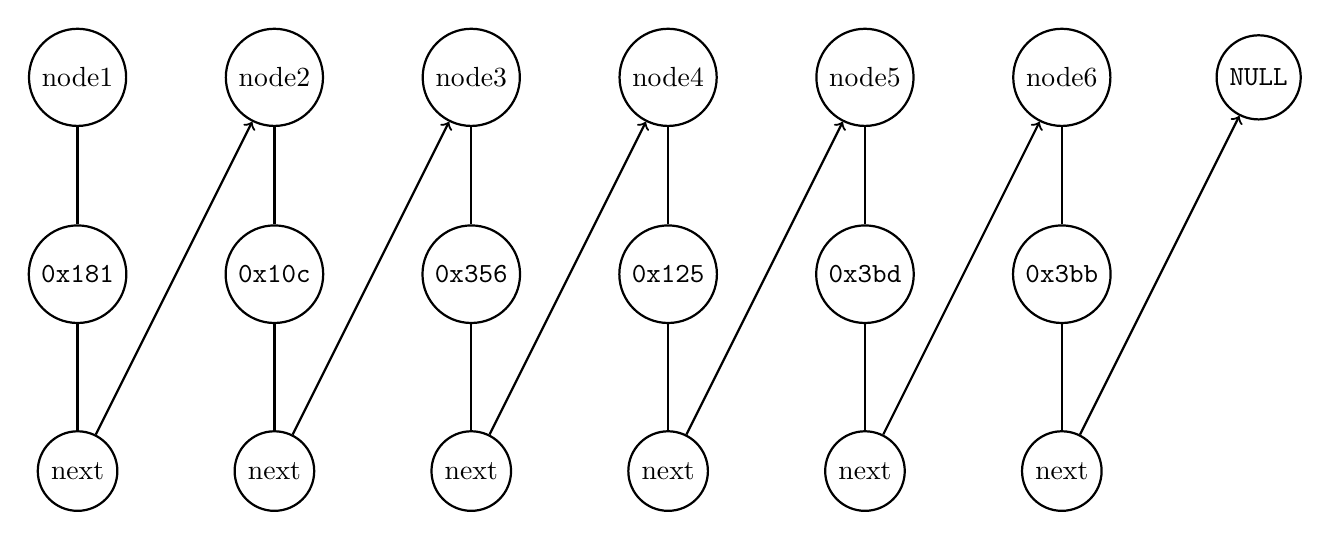
\begin{tikzpicture}[node distance={25mm}, thick, main/.style = {draw, circle}] 
    \node[main] (node1) {node$1$};
    \node[main] (val1) [below of =node1] {\verb|0x181|};
    \node[main] (next1) [below of =val1] {next};
    \node[main] (node2) [right of=node1] {node$2$};
    \node[main] (val2) [below of =node2]  {\verb|0x10c|};
    \node[main] (next2)  [below of =val2]  {next};
    \node[main] (node3) [right of=node2] {node$3$};
    \node[main] (val3) [below of =node3]  {\verb|0x356|};
    \node[main] (next3)  [below of =val3]  {next};
    \node[main] (node4) [right of=node3] {node$4$};
    \node[main] (val4) [below of =node4]  {\verb|0x125|};
    \node[main] (next4)  [below of =val4]  {next};
    \node[main] (node5) [right of=node4] {node$5$};
    \node[main] (val5) [below of =node5]  {\verb|0x3bd|};
    \node[main] (next5)  [below of =val5]  {next};
    \node[main] (node6) [right of=node5] {node$6$};
    \node[main] (val6) [below of =node6]  {\verb|0x3bb|};
    \node[main] (next6)  [below of =val6]  {next};
    \node[main] (null) [right of=node6] {\verb|NULL|};

    \draw (node1) -- (val1);
    \draw (val1) -- (next1);
    \draw[->] (next1) -- (node2);
    \draw (node2) -- (val2);
    \draw (val2) -- (next2);
    \draw[->] (next2) -- (node3);
    \draw (node3) -- (val3);
    \draw (val3) -- (next3);
    \draw[->] (next3) -- (node4);
    \draw (node4) -- (val4);
    \draw (val4) -- (next4);
    \draw[->] (next4) -- (node5);
    \draw (node5) -- (val5);
    \draw (val5) -- (next5);
    \draw[->] (next5) -- (node6);
    \draw (node6) -- (val6);
    \draw (val6) -- (next6);
    \draw[->] (next6) -- (null);
  \end{tikzpicture} 
\end{center}
This suggests the follow definition for a linked list data structure
{\renewcommand\fcolorbox[4][]{\textcolor{black}{\strut#4}}
\begin{minted}[frame=single,framesep=10pt]{c}
  struct node{
    int val, id;
    struct node *link;
  };
\end{minted}
}\noindent
Let's go back to our code, note that there's two backward jumps again, so it must be another loop.
{\renewcommand\fcolorbox[4][]{\textcolor{black}{\strut#4}}
\begin{minted}[frame=single,framesep=10pt]{c}
  if(ecx > 1){
    // Line 142
  }
  // Line 153
\end{minted}
}\noindent
Let's go to the line 142
{\renewcommand\fcolorbox[4][]{\textcolor{cyan}{\strut#4}}
\begin{minted}[frame=single,framesep=10pt]{gas}
  0x000000000040119f <+142>:   mov    0x8(%rdx),%rdx
  0x00000000004011a3 <+146>:   add    $0x1,%eax
  0x00000000004011a6 <+149>:   cmp    %ecx,%eax
  0x00000000004011a8 <+151>:   jne    0x40119f <phase_6+142>
\end{minted}
}\noindent
Let's see that's inside \verb|rdx|
{\renewcommand\fcolorbox[4][]{\textcolor{black}{\strut#4}}
\begin{minted}[frame=single,framesep=10pt]{bash}
  (gdb) x/3 $rdx
  0x6032f0 <node1>: 0x00000181 0x00000001 0x00603300
\end{minted}
}\noindent
which is the first node in our linked list, and \verb|0x8(%rdx)| is the address of the next node, to which we move. Then, \verb|eax| is incremented, and compared with \verb|ecx|, if it is not equal, loop back to the line $142$, if they are equal continue to line $153$. These lines are finding the node in the position specified in our inputs.
{\renewcommand\fcolorbox[4][]{\textcolor{cyan}{\strut#4}}
\begin{minted}[frame=single,framesep=10pt]{gas}
  0x00000000004011aa <+153>:   mov    %rdx,(%rsp,%rsi,8)
  0x00000000004011ae <+157>:   add    $0x1,%rsi
  0x00000000004011b2 <+161>:   cmp    $0x6,%rsi
  0x00000000004011b6 <+165>:   je     0x4011cd <phase_6+188>
\end{minted}
}\noindent
First, it moves the value of our current node into the address \verb|(%rsp,%rsi,8)|, and then increment \verb|rsi|, then continues the loop until $\verb|rsi| = 6$. After the loop is terminated, we go into the line $188$.
{\renewcommand\fcolorbox[4][]{\textcolor{cyan}{\strut#4}}
\begin{minted}[frame=single,framesep=10pt]{gas}
  0x00000000004011cd <+188>:   mov    (%rsp),%rbx
  0x00000000004011d1 <+192>:   mov    0x8(%rsp),%rax
  0x00000000004011d6 <+197>:   mov    %rax,0x8(%rbx)
  0x00000000004011da <+201>:   mov    0x10(%rsp),%rdx
  0x00000000004011df <+206>:   mov    %rdx,0x8(%rax)
  0x00000000004011e3 <+210>:   mov    0x18(%rsp),%rax
  0x00000000004011e8 <+215>:   mov    %rax,0x8(%rdx)
  0x00000000004011ec <+219>:   mov    0x20(%rsp),%rdx
  0x00000000004011f1 <+224>:   mov    %rdx,0x8(%rax)
  0x00000000004011f5 <+228>:   mov    0x28(%rsp),%rax
  0x00000000004011fa <+233>:   mov    %rax,0x8(%rdx)
  0x00000000004011fe <+237>:   movq   $0x0,0x8(%rax)
  0x0000000000401206 <+245>:   mov    $0x5,%ebp
  0x000000000040120b <+250>:   jmp    0x401216 <phase_6+261>
\end{minted}
}\noindent
Note that \verb|rsp| here is holding our values of the linked list. Let's inspect them, using the following custom function in \verb|gdb|.
{\renewcommand\fcolorbox[4][]{\textcolor{black}{\strut#4}}
\begin{minted}[frame=single,framesep=10pt]{bash}
  define pa
    set var $i = 1
    while $i <= 6
      printf "a[%d] = %x\n", $i, **(int*)($arg0 + 0x8*($i-1))
      set var $i = $i + 1
    end
  end
\end{minted}
}\noindent
Using this custom command with an argument of \verb|rsp|, we obtain the following
{\renewcommand\fcolorbox[4][]{\textcolor{black}{\strut#4}}
\begin{minted}[frame=single,framesep=10pt]{bash}
  (gdb) pa $rsp
  a[1] = 0x3bb
  a[2] = 0x3bd
  a[3] = 0x125
  a[4] = 0x356
  a[5] = 0x10c
  a[6] = 0x181
\end{minted}
}\noindent
The value now is shuffled according to our modified input, i.e. ``6 5 4 3 2 1''. Meaning, the first value is the value of \verb|node6|, the second value is the value of \verb|node5|, and so on. These lines just move all the data from \verb|rsp| to \verb|rbx|. Now, let's see the last few lines
{\renewcommand\fcolorbox[4][]{\textcolor{cyan}{\strut#4}}
\begin{minted}[frame=single,framesep=10pt]{gas}
  0x000000000040120b <+250>:   jmp    0x401216 <phase_6+261>
  0x000000000040120d <+252>:   mov    0x8(%rbx),%rbx
  0x0000000000401211 <+256>:   sub    $0x1,%ebp
  0x0000000000401214 <+259>:   je     0x401227 <phase_6+278>
  0x0000000000401216 <+261>:   mov    0x8(%rbx),%rax
  0x000000000040121a <+265>:   mov    (%rax),%eax
  0x000000000040121c <+267>:   cmp    %eax,(%rbx)
  0x000000000040121e <+269>:   jge    0x40120d <phase_6+252>
  0x0000000000401220 <+271>:   callq  0x401451 <explode_bomb>
  0x0000000000401225 <+276>:   jmp    0x40120d <phase_6+252>
\end{minted}
}\noindent
Firstly, we start at the line 261. Here, \verb|eax| is holding our second value, i.e. \verb|a[2]|. Then, the bomb compares \verb|a[1]| and \verb|a[2]|, if $a[1] \geq a[2]$ then we continue with our loop, otherwise, the bomb will explode. In the next iterations, the bomb also compares the current value with the next value, i.e. it is checking whether $a[i] \geq a[i + 1]$, if there exists an $i$ that violates the condition, the bomb will detonate, otherwise, it jumps peacefully to the line 278, which is the end of our function.
{\renewcommand\fcolorbox[4][]{\textcolor{cyan}{\strut#4}}
\begin{minted}[frame=single,framesep=10pt]{gas}
  0x0000000000401227 <+278>:   add    $0x50,%rsp
  0x000000000040122b <+282>:   pop    %rbx
  0x000000000040122c <+283>:   pop    %rbp
  0x000000000040122d <+284>:   pop    %r12
  0x000000000040122f <+286>:   pop    %r13
  0x0000000000401231 <+288>:   pop    %r14
  0x0000000000401233 <+290>:   retq
\end{minted}
}\noindent
In conclusion, the last few lines are checking if our values from the array ``\verb|a|'' is nonincreasing. If it is, then we defuse the bomb, otherwise, the bomb will detonate. In our case of dummy input, the bomb will detonate after it detects $a[1] < a[2]$, which violates the condition. Therefore, we have to find a permutation of $\{1, 2, 3, 4, 5, 6\}$ so that our final ``array'' is nonincreasing. Recall that the original values of the nodes are
\begin{center}
  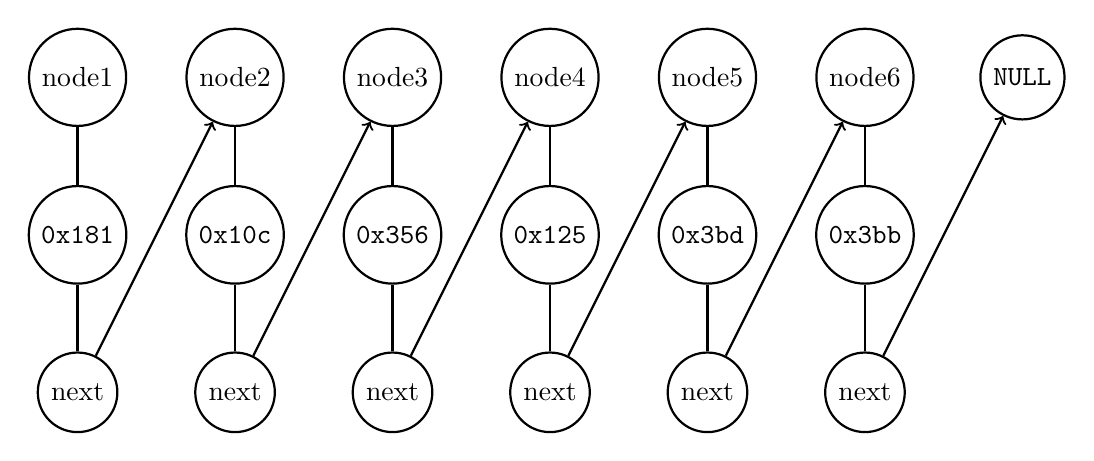
\begin{tikzpicture}[node distance={20mm}, thick, main/.style = {draw, circle}] 
    \node[main] (node1) {node$1$};
    \node[main] (val1) [below of =node1] {\verb|0x181|};
    \node[main] (next1) [below of =val1] {next};
    \node[main] (node2) [right of=node1] {node$2$};
    \node[main] (val2) [below of =node2]  {\verb|0x10c|};
    \node[main] (next2)  [below of =val2]  {next};
    \node[main] (node3) [right of=node2] {node$3$};
    \node[main] (val3) [below of =node3]  {\verb|0x356|};
    \node[main] (next3)  [below of =val3]  {next};
    \node[main] (node4) [right of=node3] {node$4$};
    \node[main] (val4) [below of =node4]  {\verb|0x125|};
    \node[main] (next4)  [below of =val4]  {next};
    \node[main] (node5) [right of=node4] {node$5$};
    \node[main] (val5) [below of =node5]  {\verb|0x3bd|};
    \node[main] (next5)  [below of =val5]  {next};
    \node[main] (node6) [right of=node5] {node$6$};
    \node[main] (val6) [below of =node6]  {\verb|0x3bb|};
    \node[main] (next6)  [below of =val6]  {next};
    \node[main] (null) [right of=node6] {\verb|NULL|};

    \draw (node1) -- (val1);
    \draw (val1) -- (next1);
    \draw[->] (next1) -- (node2);
    \draw (node2) -- (val2);
    \draw (val2) -- (next2);
    \draw[->] (next2) -- (node3);
    \draw (node3) -- (val3);
    \draw (val3) -- (next3);
    \draw[->] (next3) -- (node4);
    \draw (node4) -- (val4);
    \draw (val4) -- (next4);
    \draw[->] (next4) -- (node5);
    \draw (node5) -- (val5);
    \draw (val5) -- (next5);
    \draw[->] (next5) -- (node6);
    \draw (node6) -- (val6);
    \draw (val6) -- (next6);
    \draw[->] (next6) -- (null);
  \end{tikzpicture} 
\end{center}
After sorting, the nodes will be in the following order
\begin{center}
  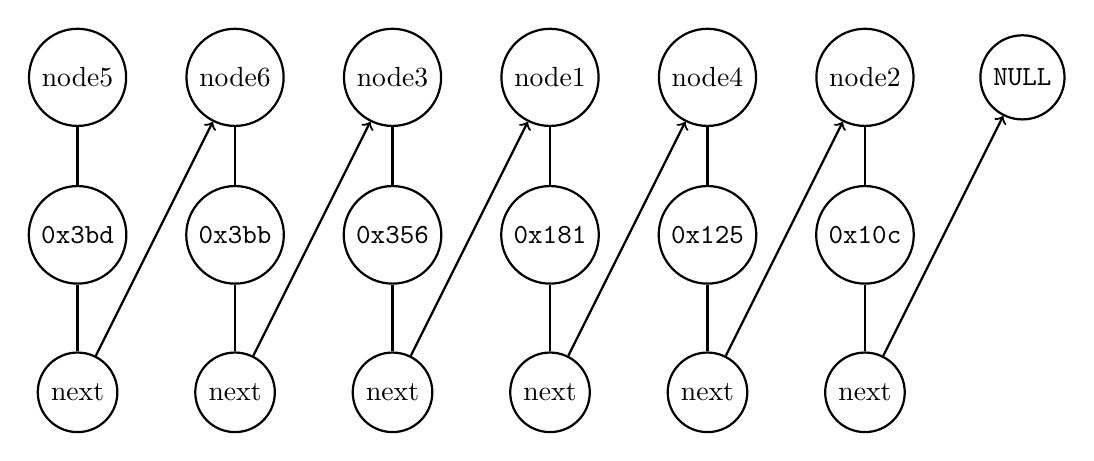
\begin{tikzpicture}[node distance={20mm}, thick, main/.style = {draw, circle}] 
    \node[main] (node1) {node$5$};
    \node[main] (val1) [below of =node1] {\verb|0x3bd|};
    \node[main] (next1) [below of =val1] {next};
    \node[main] (node2) [right of=node1] {node$6$};
    \node[main] (val2) [below of =node2]  {\verb|0x3bb|};
    \node[main] (next2)  [below of =val2]  {next};
    \node[main] (node3) [right of=node2] {node$3$};
    \node[main] (val3) [below of =node3]  {\verb|0x356|};
    \node[main] (next3)  [below of =val3]  {next};
    \node[main] (node4) [right of=node3] {node$1$};
    \node[main] (val4) [below of =node4]  {\verb|0x181|};
    \node[main] (next4)  [below of =val4]  {next};
    \node[main] (node5) [right of=node4] {node$4$};
    \node[main] (val5) [below of =node5]  {\verb|0x125|};
    \node[main] (next5)  [below of =val5]  {next};
    \node[main] (node6) [right of=node5] {node$2$};
    \node[main] (val6) [below of =node6]  {\verb|0x10c|};
    \node[main] (next6)  [below of =val6]  {next};
    \node[main] (null) [right of=node6] {\verb|NULL|};

    \draw (node1) -- (val1);
    \draw (val1) -- (next1);
    \draw[->] (next1) -- (node2);
    \draw (node2) -- (val2);
    \draw (val2) -- (next2);
    \draw[->] (next2) -- (node3);
    \draw (node3) -- (val3);
    \draw (val3) -- (next3);
    \draw[->] (next3) -- (node4);
    \draw (node4) -- (val4);
    \draw (val4) -- (next4);
    \draw[->] (next4) -- (node5);
    \draw (node5) -- (val5);
    \draw (val5) -- (next5);
    \draw[->] (next5) -- (node6);
    \draw (node6) -- (val6);
    \draw (val6) -- (next6);
    \draw[->] (next6) -- (null);
  \end{tikzpicture} 
\end{center}
Thus, the correct permutation should be $\{5, 6, 3, 1, 4, 2\}$.However, note that before shuffling the linked list, our input is modified by the function
$$ f(x) = 7 - x $$
Therefore, the correct input should be ``\verb|2 1 4 6 3 5|''. Resetting the bomb and typing in the correct string, we have successfully defused the entire bomb!
{\renewcommand\fcolorbox[4][]{\textcolor{black}{\strut#4}}
\begin{minted}[frame=single,framesep=10pt]{text}
  [edusc03-052@cheetah022 bomb52]$ ./bomb input.txt
  Welcome to my fiendish little bomb. You have 6 phases with
  which to blow yourself up. Have a nice day!
  Phase 1 defused. How about the next one?
  That's number 2.  Keep going!
  Halfway there!
  So you got that one.  Try this one.
  Good work!  On to the next...
  2 1 4 6 3 5
  Congratulations! You've defused the bomb!
\end{minted}
}\noindent



\newpage



\end{document}
